\subsection{Consolidamento dei requisiti}

\subsubsection{Prospetto orario}
Nel periodo di consolidamento dei requisiti la distribuzione oraria è la seguente:

\renewcommand{\arraystretch}{1.5}
\begin{table}[H]
\begin{center}
\begin{tabular}{|c|c|c|c|c|c|c|c|}
\hline
\rowcolor{title_row}
\textbf{\color{title_text}{Nome}} & \textbf{\color{title_text}{Resp.}} & \textbf{\color{title_text}{Ammi.}} & \textbf{\color{title_text}{Analist.}} & \textbf{\color{title_text}{Progett.}} & \textbf{\color{title_text}{Program.}} & \textbf{\color{title_text}{Verific.}} & \textbf{\color{title_text}{Totale}} \\ \hline
Andrea Trevisin  & 5 & 2 & & & & & 7 \\ \hline
Giacomo Barzon   & & & 3 & & & 3 & 6 \\ \hline
Giovanni Sorice  & & 5 & & & & 1 & 6 \\ \hline
Lorenzo Busin    & 5 & 1 & 4 & & & & 10 \\ \hline
Marco Costantino & & & 3 & & & 5 & 8 \\ \hline
Michele Roverato & & & 3 & & & 5 & 8 \\ \hline
Nicolò Tartaggia & & 3 & & & & 5 & 8 \\ \hline
\end{tabular}
\caption{Tabella 5.2.1: Distribuzione oraria del periodo "Consolidamento dei requisiti"\label{}}
\end{center}
\end{table}
\renewcommand{\arraystretch}{1}

Il seguente grafico dà una rappresentazione visiva della suddivisione oraria: \\
\begin{figure} [H]
	\centering
	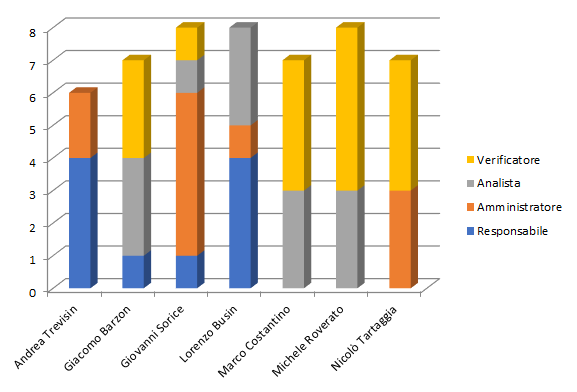
\includegraphics[scale=1]{Res/ExcelGrafici/Grafici/ConsolidamentoOre.png}
	\caption{Figura 5.2.1: Grafico suddivisione oraria del periodo "Consolidamento dei requisiti"}\label{}
\end{figure}


\subsubsection{Prospetto economico}
Nel periodo di consolidamento dei requisiti il resoconto della distribuzione delle ore e dei relativi costi è la seguente:

\renewcommand{\arraystretch}{1.5}
\begin{table}[H]
\begin{center}
\begin{tabular}{|c|c|c|}
\hline
\rowcolor{title_row}
\textbf{\color{title_text}{Ruolo}}  & \textbf{\color{title_text}{Ore}} & \textbf{\color{title_text}{Costo in \euro}} \\ \hline
Responsabile    & 10 & 300 \\ \hline
Amministratore  & 11 & 220 \\ \hline
Analista        & 13 & 325 \\ \hline
Progettista     & & \\ \hline
Programmatore   & & \\ \hline
Verificatore    & 19 & 285 \\ \hline
\textbf{Totale} & \textbf{53}    & \textbf{1.130}    \\ \hline
\end{tabular}
\caption{Tabella 5.2.2: Prospetto economico del periodo "Consolidamento dei requisiti"\label{}}
\end{center}
\end{table}
\renewcommand{\arraystretch}{1}

Il seguente grafico dà una rappresentazione visiva della distribuzione dei ruoli: \\
\begin{figure} [H]
	\centering
	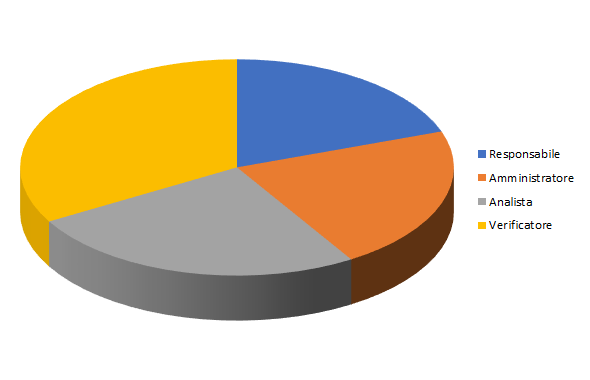
\includegraphics[scale=1]{Res/ExcelGrafici/Grafici/ConsolidamentoRuoli.png}
	\caption{Figura 5.2.2: Grafico suddivisione dei ruoli del periodo "Consolidamento dei requisiti"}\label{}
\end{figure}

\pagebreak
